%
% problemstellung.tex -- Beispiel-File für die Beschreibung des Problems
%
% (c) 2020 Prof Dr Andreas Müller, Hochschule Rapperswil
%
\section{Problemstellung
\label{vanderpol:section:problemstellung}}
\rhead{Problemstellung}
Um einen chaotischen Verlauf zu finden, ist es notwendig, zunächst die Differentialfunktion und ihre Repräsentationen zu untersuchen.
Die Van-der-Pol-Gleichung (Gl. \ref{vanderpol:equations:vdp}) ist eine \textbf{nichtlineare} Differentialgleichung zweiter Ordnung. 
Die Nichtlinearität wird durch die Tatsache festgelegt, dass der Koeffizient multipliziert mit $\dot{x}$ nicht linear ist, sondern von der Funktion selbst abhängt.
Im Vergleich dazu hat eine lineare Differentialgleichung zweiter Ordnung nur konstante Koeffizienten, wie z.B. die RLC-Schwingkreise DGL:
\begin{equation*}
	LC \frac{d^{2} i}{d t^{2}}+RC \frac{d i}{d t}+i
\end{equation*}

\subsection{Homogene gleichung
\label{vanderpol:subsection:homogene}}
Die Differentialgleichung wird als homogen bezeichnet, wenn sie auf Null gesetzt ist.
\begin{equation}
	\ddot{x} - \mu \left(1-x^{2}\right)\dot{x}+x = 0
\label{vanderpol:equations:homogene}
\end{equation}
Es ist möglich, die Gleichung mit der folgenden Ersetzung auf den ersten Grad zu reduzieren, so dass sie mithilfe numerischer Lösungsmethoden aufgelöst werden kann.
\begin{align}
	\dot{x} &= y  \label{vanderpol:equations:homogene_1} \\
	\dot{y} &= \mu \left(1-x^{2}\right)y - x 
	\label{vanderpol:equations:homogene_2}
\end{align}
Die Funktion neigt dazu, nach einer bestimmten Zeit in einer bestimmten Trajektorien zu oszillieren, unabhängig vom Anfangswert. Diese Orbit wird Grenzzyclus oder ``Limit Cycle'' genannt. Mit dem Parameter $\mu$ wird die Form der Umlaufbahn verändert. Es ist interessant zu bemerken, dass bei $\mu = 0$ die Gleichung $\ddot{x} + x = 0$ wird, nämlich eine linear harmonische Schwingung.
\begin{figure}[ht]
	\centering
	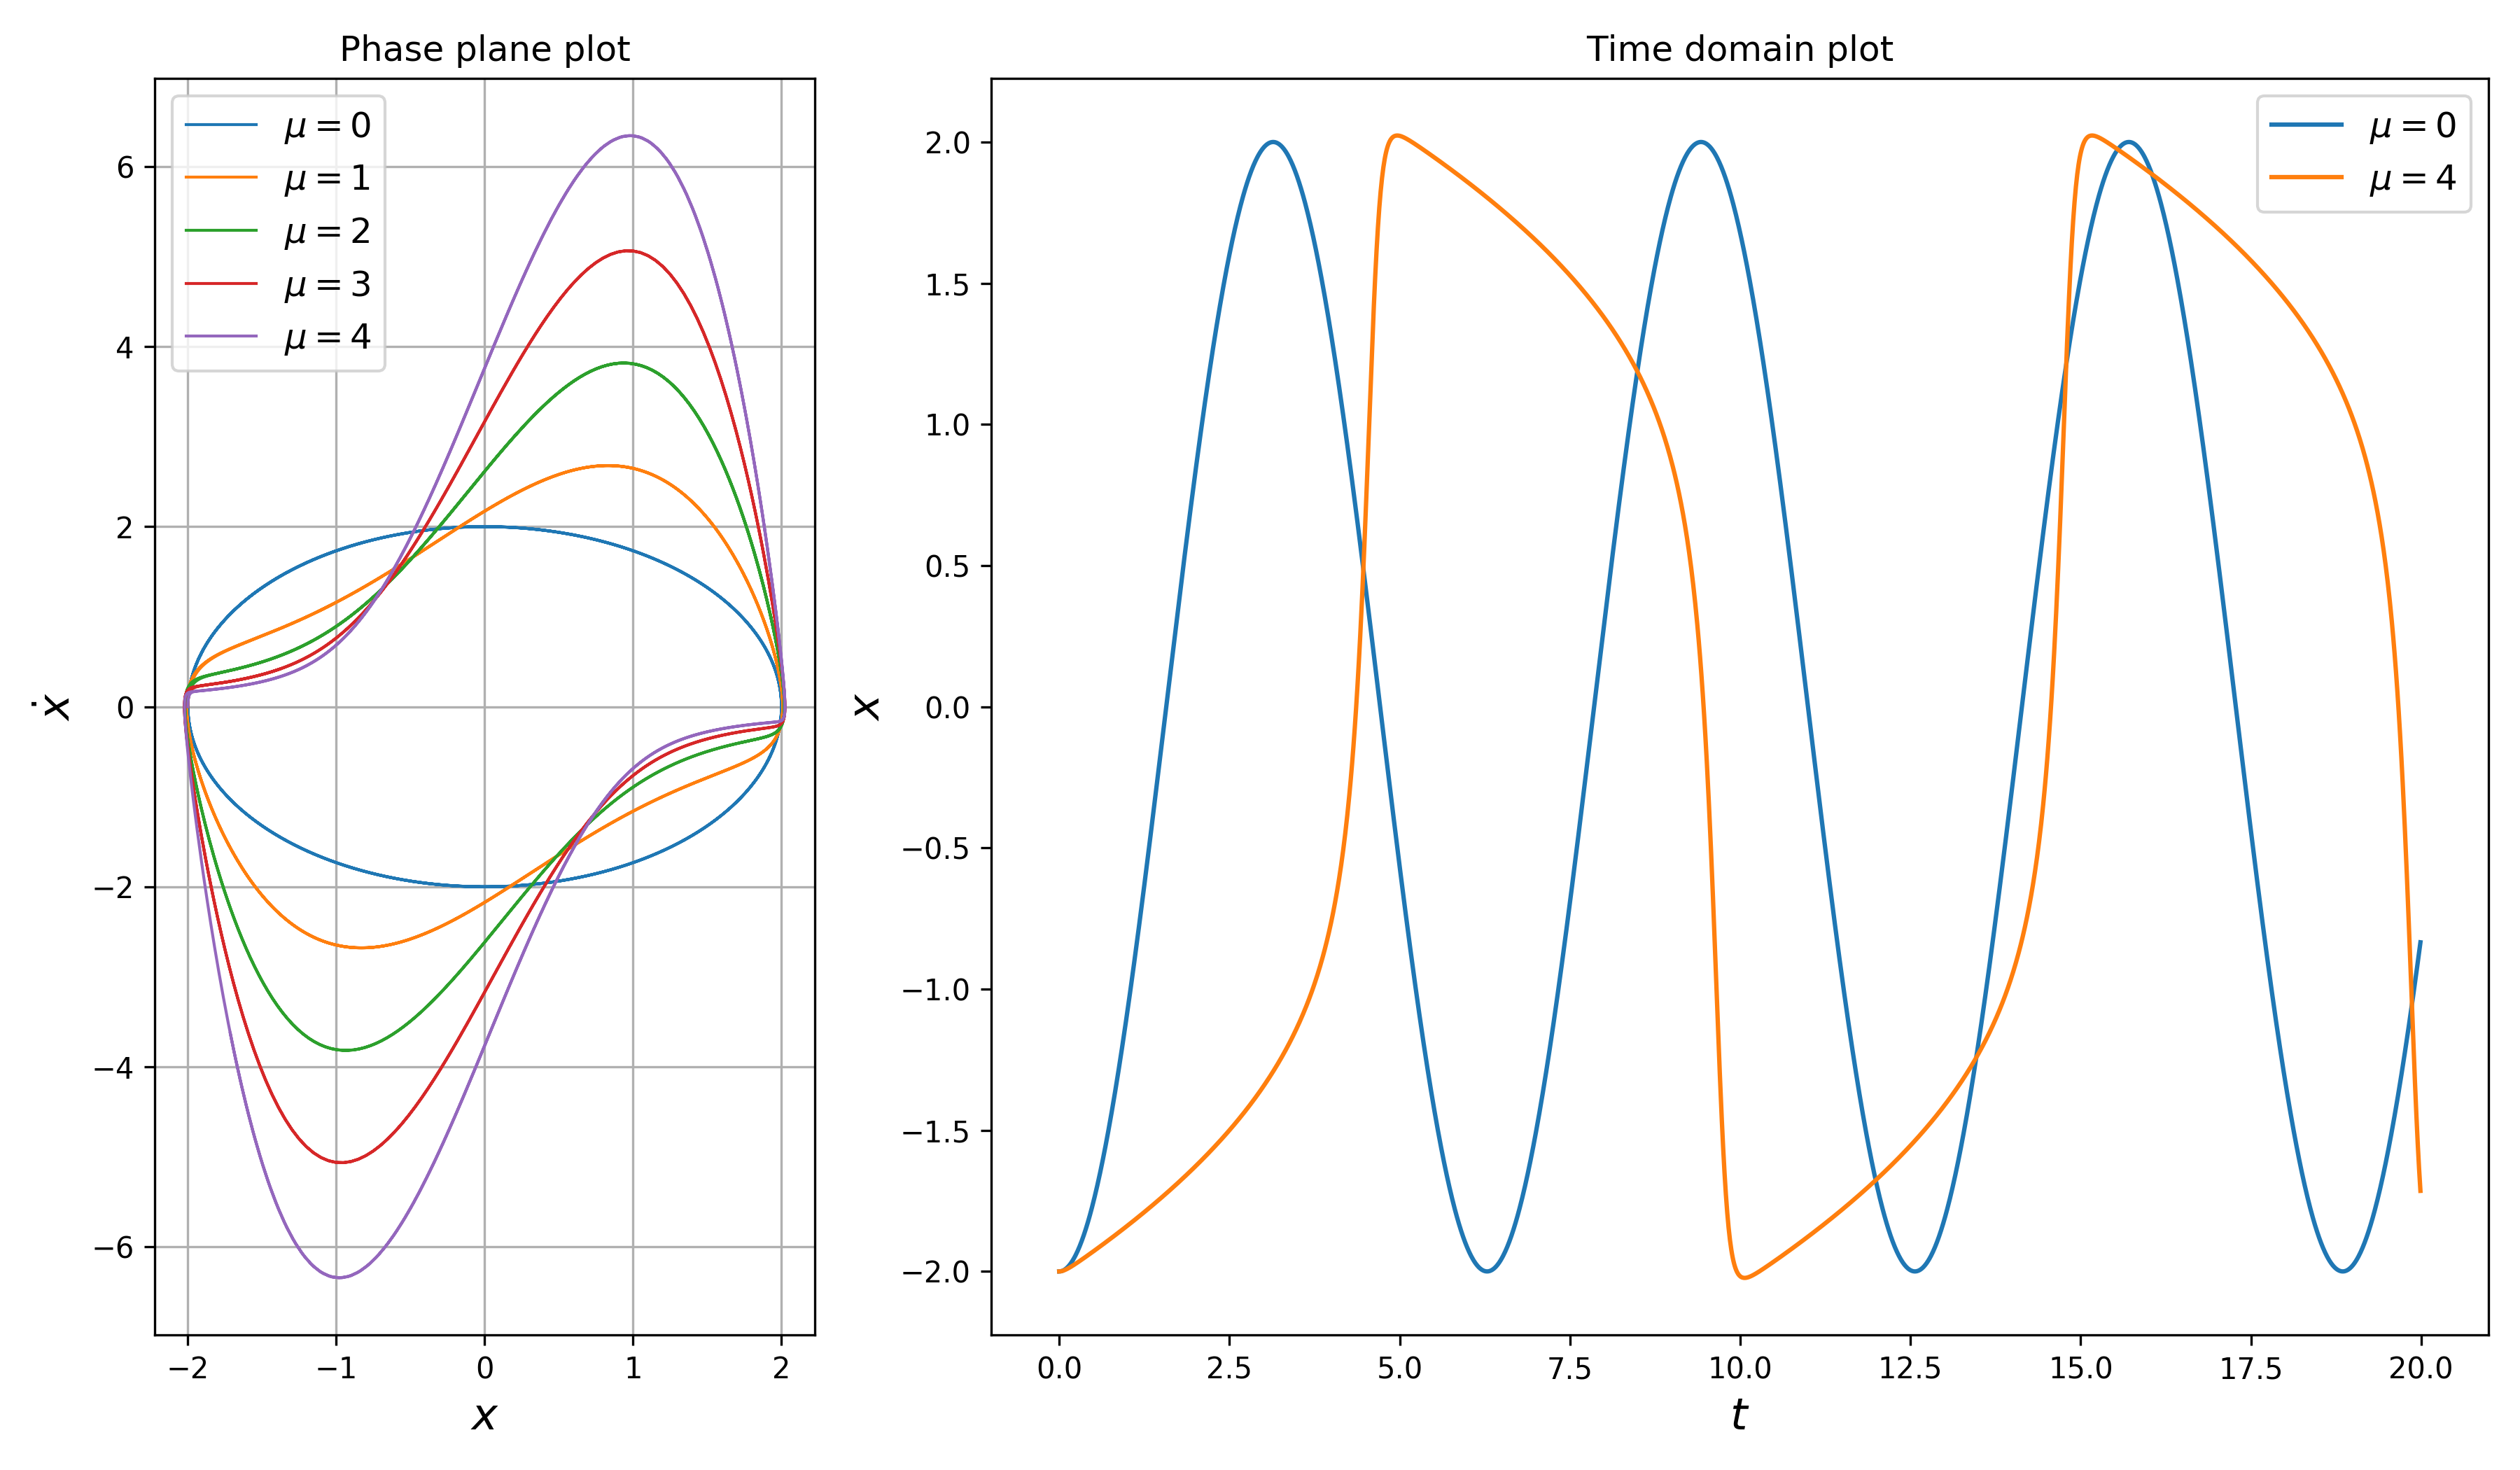
\includegraphics[width=\textwidth]{papers/vanderpol/figures/homogene_plot.png}
	\caption{Phase und Zeit-Raum-Diagramm mit verschiedenen $\mu$\label{vanderpol:figures:homogene}}
\end{figure}

\noindent Die homogene Van-der-Pol-Gleichung ist stabil und zeigt \textbf{kein} chaotisches Verhalten.
\subsection{Inhomogene gleichung}
\label{vanderpol:subsection:inhomogene}
Um einen chaotischen Verlauf zu beobachten, ist es daher notwendig, die inhomogene Gleichung zu untersuchen.
\begin{equation*}
	\ddot{x}-\mu\left(1-x^{2}\right) \dot{x}+x =\textcolor{red}{f(x)}
\label{vanderpol:equations:inhomogene_gen}
\end{equation*}
Durch die Einstellung $f(x) = A \sin(\omega t)$ wird die Gleichung zur sogenannten ``Forced Van-der-Pol equation''.
\begin{equation}
	\ddot{x}-\mu\left(1-x^{2}\right) \dot{x}+x = A \sin(\omega t)
\label{vanderpol:equations:inhomogene_sin}
\end{equation}
In der praktischen Anwendung ist es so, wie wenn man einen Wechselstromgenerator an den Oszillator anschliesst. Wie vorher geschehen (Gl. \ref{vanderpol:equations:homogene_1} und  \ref{vanderpol:equations:homogene_2}), wird die Differentialgleichung auf die erste Ordnung reduziert, um eine numerische Lösung zu erhalten.
\begin{align}
\dot{x} &= y \label{vanderpol:equations:inhomogene_1} \\
\dot{y} &= \mu\left(1-x^{2}\right) y - x + A \sin(\omega t)
\label{vanderpol:equations:inhomogene_2}
\end{align}
Die Änderung der Amplitude $A$ verändert das Systemverhalten. Bei der Beobachtung der Frequenz des Oszillators wurden drei verschiedene Fälle erkannt. Wie in der Abb. \ref{vanderpol:figures:fft} gezeigt, ist die Frequenz des Van-der-Pol-Oszillators dominant, wenn der $A$-Wert kleiner als der kritische Wert ist. Wenn der Wert höher ist, dominiert die $\omega$-Frequenz. Durch Setzen der Werte $\mu=0,2$ und $\omega=1,15$ beträgt der kritische Wert von $A$ in diesem Fall $0.32$.
\begin{figure}[ht]
	\centering
	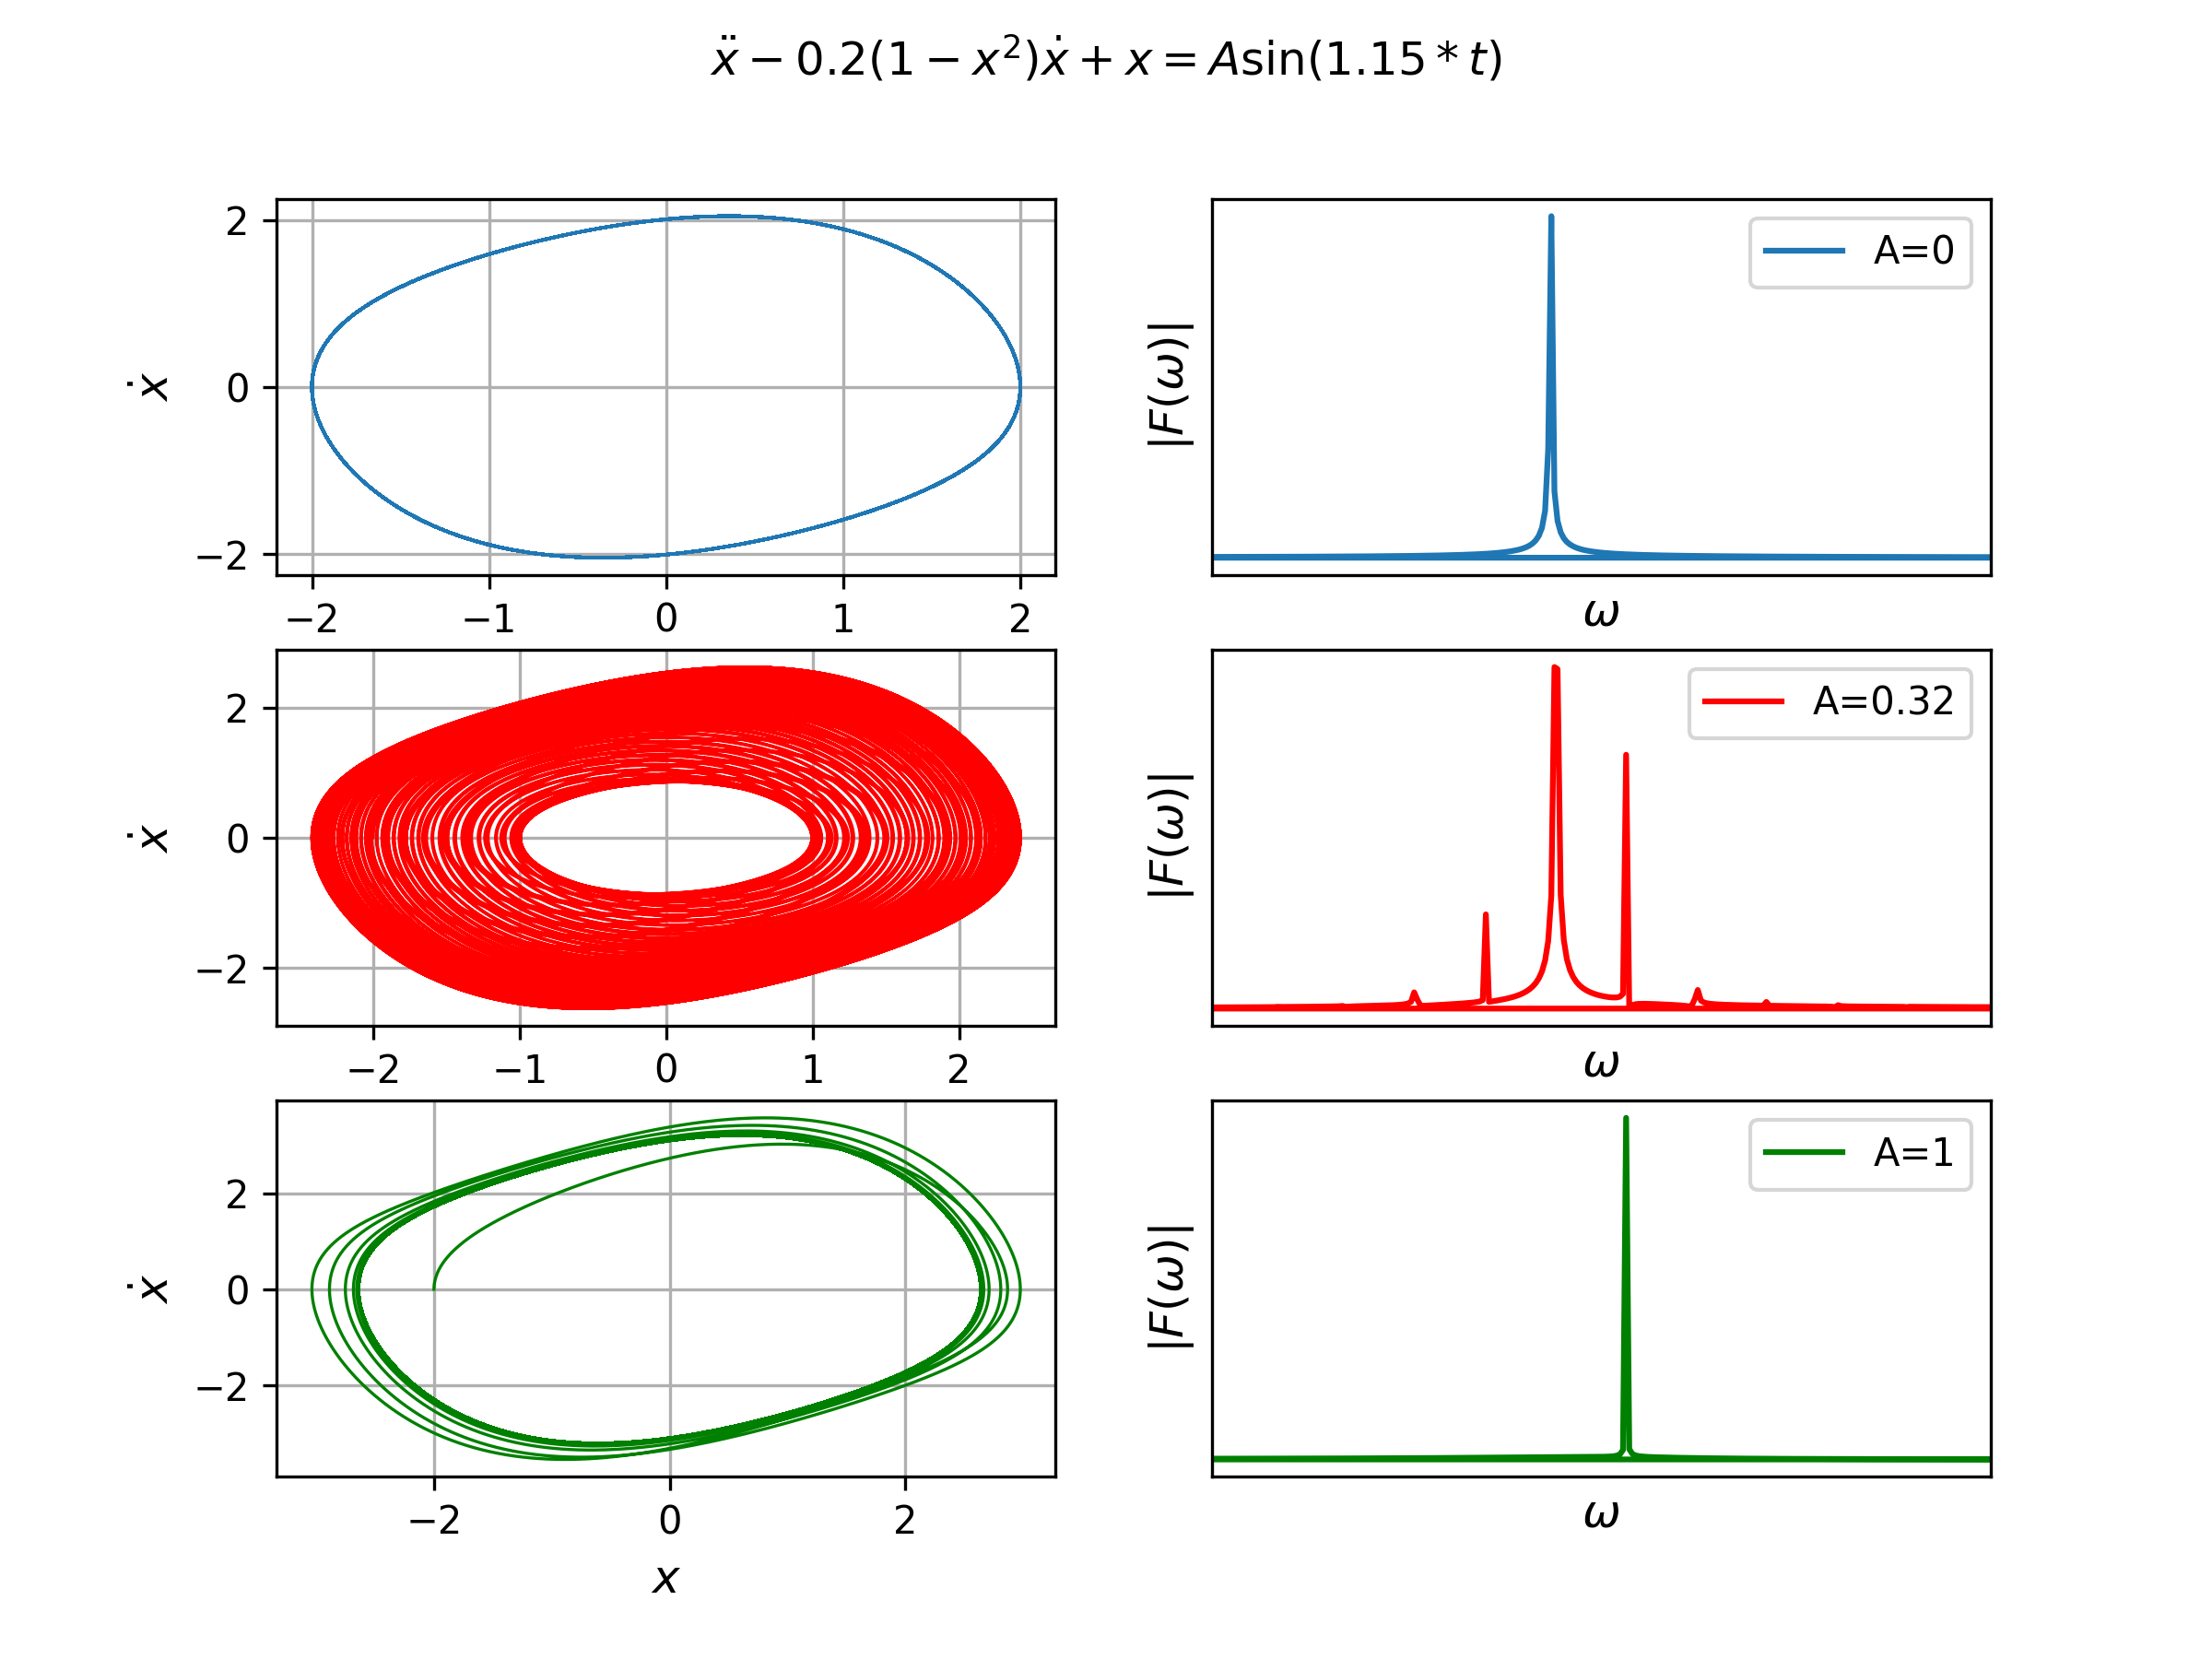
\includegraphics[width=\textwidth]{papers/vanderpol/figures/fft_plot.png}
	\caption{\todo{}\label{vanderpol:figures:fft}}
\end{figure}
\todo{continuare capitolo}

\subsection{Chaos}
\label{vanderpol:subsection:chaos}
 
\begin{cquote}[30pt]{Edward Lorenz}
``Chaos: When the present determines the future, but the approximate present does not approximately determine the future.''
\end{cquote}
 
\subsubsection{Anfangsbedingung}
\label{vanderpol:subsubsection:anfangsbedingung}
 
Das angeführte Zitat ist genau die Definition, die das in diesem Kapitel untersuchte Problem erklärt, nämlich die Instabilität der numerischen Methoden. Letztere führen einen Rundungsfehler ein, der sich während der verschiedenen Iterationen ansammelt und zu völlig unterschiedlichen Lösungen führt. Dies kann auch nach einer bestimmten Zeitspanne geschehen.
Etwas Ähnliches geschieht, wenn, immer in einem chaotischen System, eine kleine Variation der Anfangsbedingungen eingeführt wird.  Dieser kleine Unterschied kann, wie oben beschrieben, das langfristige Verhalten des Systems stark beeinflussen. Dieser Effekt wird auch als " Butterfly-Effekt " bezeichnet. Zur Erklärung dieses Phänomens verwendete Edward Lorentz in 1972 auf einer Konferenz diesen Satz: "Ein Schmetterling schlägt in Peking mit den Flügeln, und in New York kommt Regen statt Sonne". Kann eine solch minimale Veränderung der Anfangsbedingungen das Endergebnis vollständig verändern? Die Antwort ist offensichtlich ja, wie aus den Grafiken hervorgeht berichtet.

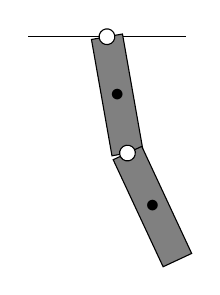
\begin{tikzpicture}
 
\draw (-1,0) -- (1,0);
 
\begin{scope}[rotate=10]
 
\draw[fill=gray]  (-0.2,0) rectangle (0.2,-1.5) node[midway](a){$\bullet$};
\draw[fill=gray, rotate around={15:(0, -1.5)}] (-0.2,-1.5) rectangle (0.2,-3)node[midway](a){$\bullet$};
\draw[fill=white] (0,-1.5) circle(0.1);
\draw[fill=white] (0,0) circle(0.1);
 
\end{scope}
 
\end{tikzpicture}
\todo{cont. Capitolo, posizionare immagine}




